\section{Higgs Combination} \label{section:higgs_combination}
To perform statistical tests in order to extract physical quantities of interest, we employ Higgs Combination Package\cite{}. It allows us to perform the various tests for each category individually (building a likelihood for a single category) and to combine all of the categories simultaneously as well (single likelihood still, but bins from all of the categories will be used for fitting). Given that we are performing a search of the SM Higgs Boson, the main objective is to improve, to lower, the expected exclusion limits that we are to put on SM Higgs production cross-section with the data collected during Run~II in 2016. In this section we thouroughly discuss the instrument, Higgs Combination Package, that is going to be utilized to derive the Exclusion Limits.

At this stage, we have built the parametric model of our signal (in terms of the floating Higgs Boson mass), performed the Fisher Test for various families and selected the actual envelope of analytic functions that will be used further. The next steps can be summarized as follows:
\begin{itemize}
    \item Build the workspaces and datacards for each category in a proper format as specified by the Higgs Combination Package. Datacard is a textual representation of the model, which specifies what signals, backgrounds, data samples are to be used.
    \item Validate models using Asimov dataset by injecting a signal of some known strength. Asimov dataset is a sample distribution generateed from a given analytical form without applying any Gaussian or Poisson randomization applied to the sampled points.
    \item Perform the relevant Statistical Tests. We are primarily interested in the Exclusion Limits computed using the Asymptotic Approximation (for a full treatment, please refer to this note\cite{}).
\end{itemize}

\subsection{Datacards and Workspaces}
The Higgs Combination Package uses datacards and workspaces where models
are defined to perform the tests. A datacard outlines our models, yields
from data, signal and background processes. In the datacard, we also list all
of the uncertainties (nuisances) that can modify the yields of our models.
Workspaces are the containers for the programmatically specified signal and
background models. The detailed list of inputs that are used in the combination
 is the following:
\begin{itemize}
    \item Mass shapes for the actual data for each category.
    \item Background models for each category. All of models come inside of an envelope (RooMultiPdf) as described earlier. The overall normalization for the background yield as well as the parameters of each functional form are left completely floating, unles they are meant to be constrained by the model.
    \item Signal models for each category and for each production process. All model parameters are parametric in the Higgs Boson mass. The purpose is to test various mass hypotheses. It is crucial to note that all of the Signal Model parameters are frozen after performing the procedure described in the earlier section~\ref{section:higgs_signalmodel}. However, they are parametric in the Higgs Boson mass.
    \item Nuisances (systematic uncertainties) that influence our measurement (integrated luminosity, pile-up, etc...) have to be considered. We provide multiplicative nuisance parameters that can modify the Standard Model Higgs yield.
\end{itemize}

\subsection{Validity Tests against Asimov}
The very first test of the validity of the model to be used is to perform the
tests against the Asimov Dataset. The tests performed can summarized in the
following procedure:
\begin{itemize}
    \item Given the signal and background models we generate an Asimov dataset with a certain signal strength, $\mu$ of $1$. This is to be done for each category individually.
    \item Perform the signal plus background fit to the generated Asimov dataset,
    \item The fitted signal strength, $\mu$, should return the value that has been injected, $1$. If substantial variations are observed, it is a clear sign of an issue with the model. One of the issues observed during such tests was the situation when background was too flexible and was able to ''eat'' some of the signal under the Higgs peak. The resolution was to increase the granularity of the mass distributions.
\end{itemize}
Figure~\ref{fig:higgs_combination_asimovtests} provides an example of a single category test against the Asimov dataset. The mass spectrum shown on the left side of the figure shows the generated dataset overlaid with the fit that was performed with the function from which the dataset was generated. On the right side, the profiling of the metric that is minimized during the fit, $-2\Delta\log{\mathcal{L}}$, versus signal strength is shown. Very good agreement is observed.
\begin{figure}[hbp]
     \centering
     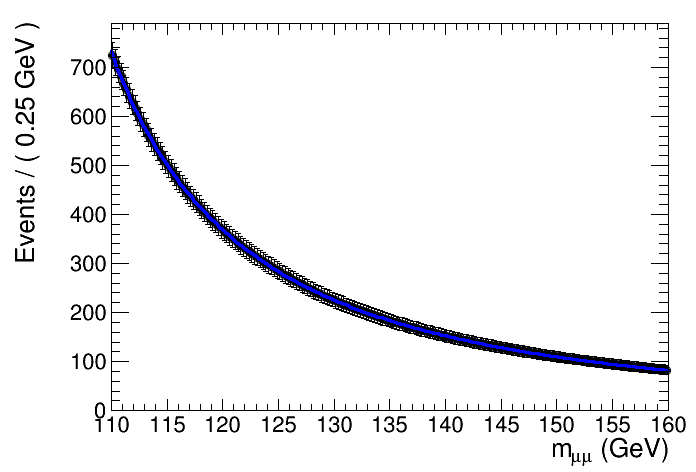
\includegraphics[width=0.7\textwidth]{figures/combine/asimovTests/cat6_x_fit_b.png}\\
     %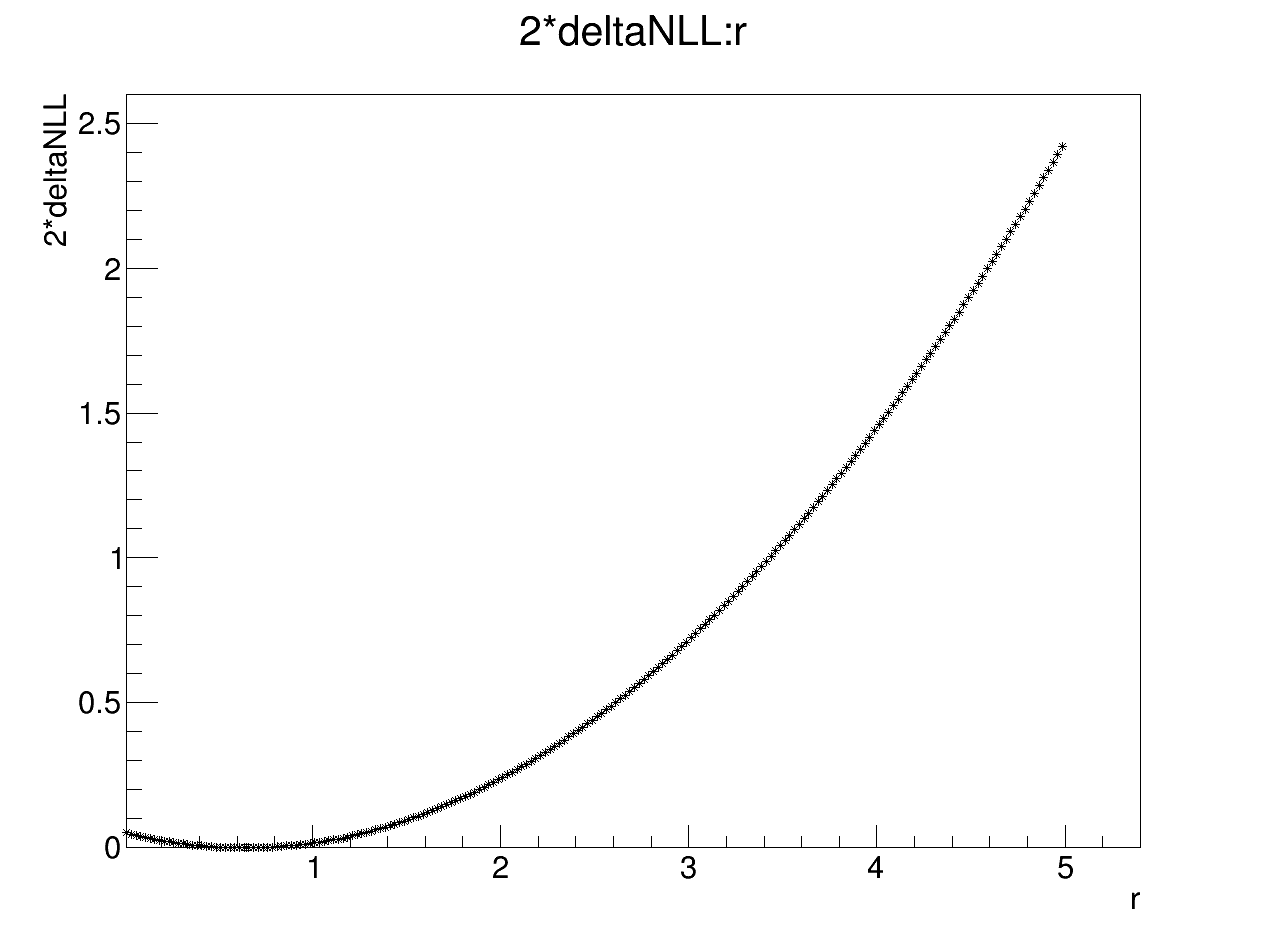
\includegraphics[width=0.3\textwidth]{figures/combine/asimovTests/NLL_asimovTest_1GeV.png}
     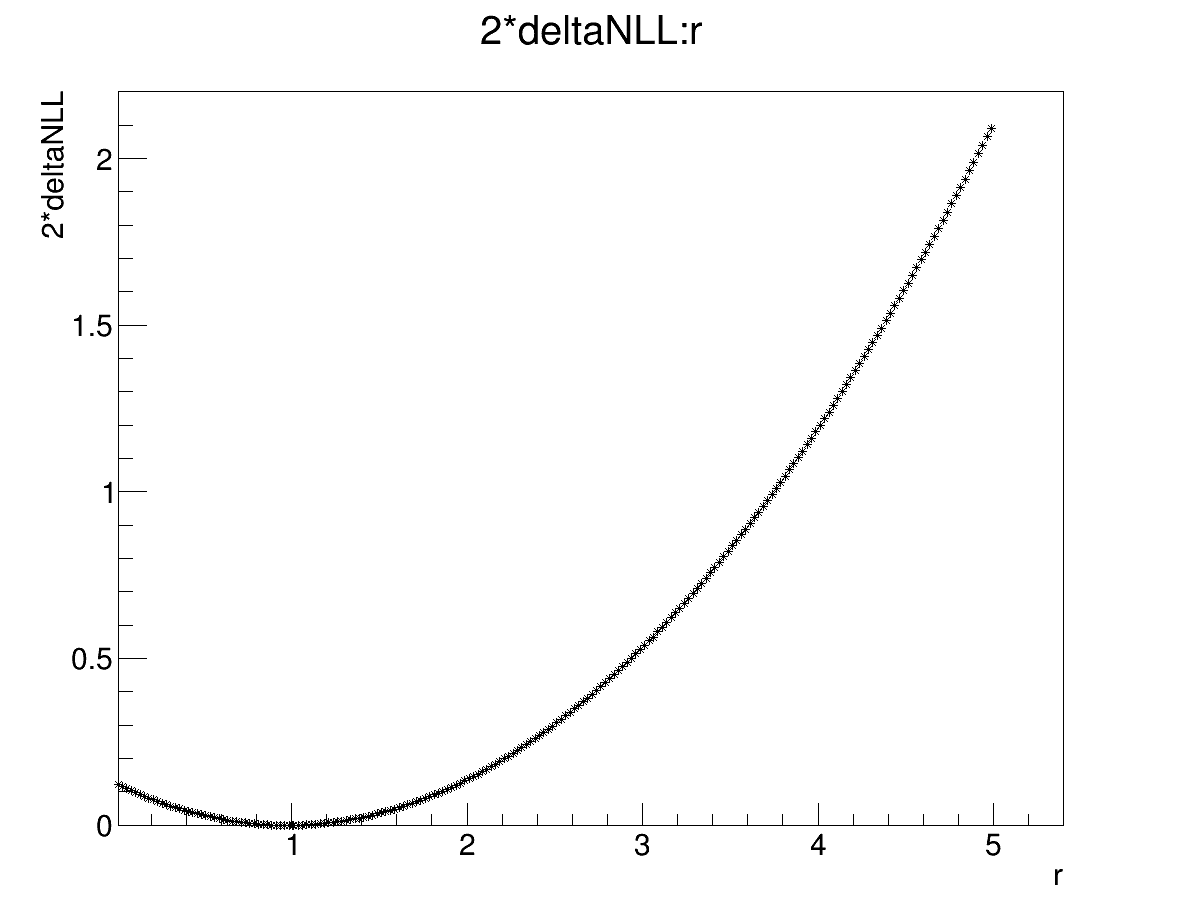
\includegraphics[width=0.7\textwidth]{figures/combine/asimovTests/NLL_asimovTest_p25GeV.png}
     \caption{The generated Asimov dataset fitted with the same functional form it was generated with (top). Must show perfect match. The $-2\Delta\log{\mathcal{L}}$ versus $\mu$ (Higgs Combination Package uses r for $\mu$) profiling (bottom). The minimum is very close to $1$ ($> 0.99$), which confirms the validity of the model. The plot is asymmetric and shifted to the positive values of the signal strength on purpose as negative values are not physical.}
     \label{fig:higgs_combination_asimovtests}
 \end{figure}

\subsection{Exclusion Limits}
The physical quantity of interest that we are to compute is the 95\% Confidence Level (CL) upper exclusion limits, computed using Asymptotic approximation (consult \cite{} for a thourough treatment), that are to be placed on the Standard Model Higgs Boson production cross-section. As it was already mentioned, Higgs Combination package is used for computating physics quantities of interest and it allows to transparently combine all of the categories.
% The analysis is optimzed against the 95\% Confidence Level (CL) upper limits that we place on the SM production cross-section of the Higgs boson.
% Expected limits are computed using the asymptotic approximation.

% Figure~\ref{combine:LimitsAsymptotic} shows the expected exclusion limit computed using asymptotic approximation on the Asimov dataset
% as a function of the probed Higgs boson mass and for the combination of all event categories as defined in Run~I analysis.

% %The left plot shows limits for Higgs mass of $\mH=125\,\gev$ only but across all of the categories and various combinations.
% %The right one shows exclusion limits as a function of the probed Higgs Mass and for a combination of all of the categories.

% \begin{figure}[hbp]
%      \centering
%      %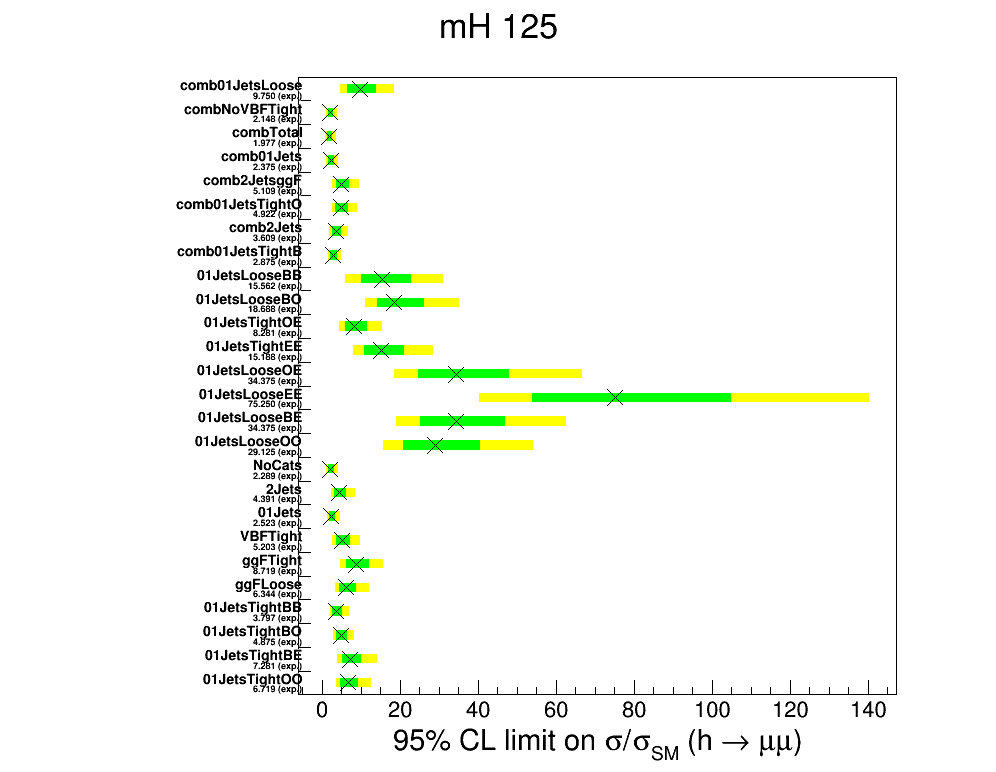
\includegraphics[width=0.45\textwidth]{figures/combine/limitsAsymptotic/baseline_110to160_p25GeV_NoNuis_Viktor/limitsByMass__125__TripleGaus.png}
%       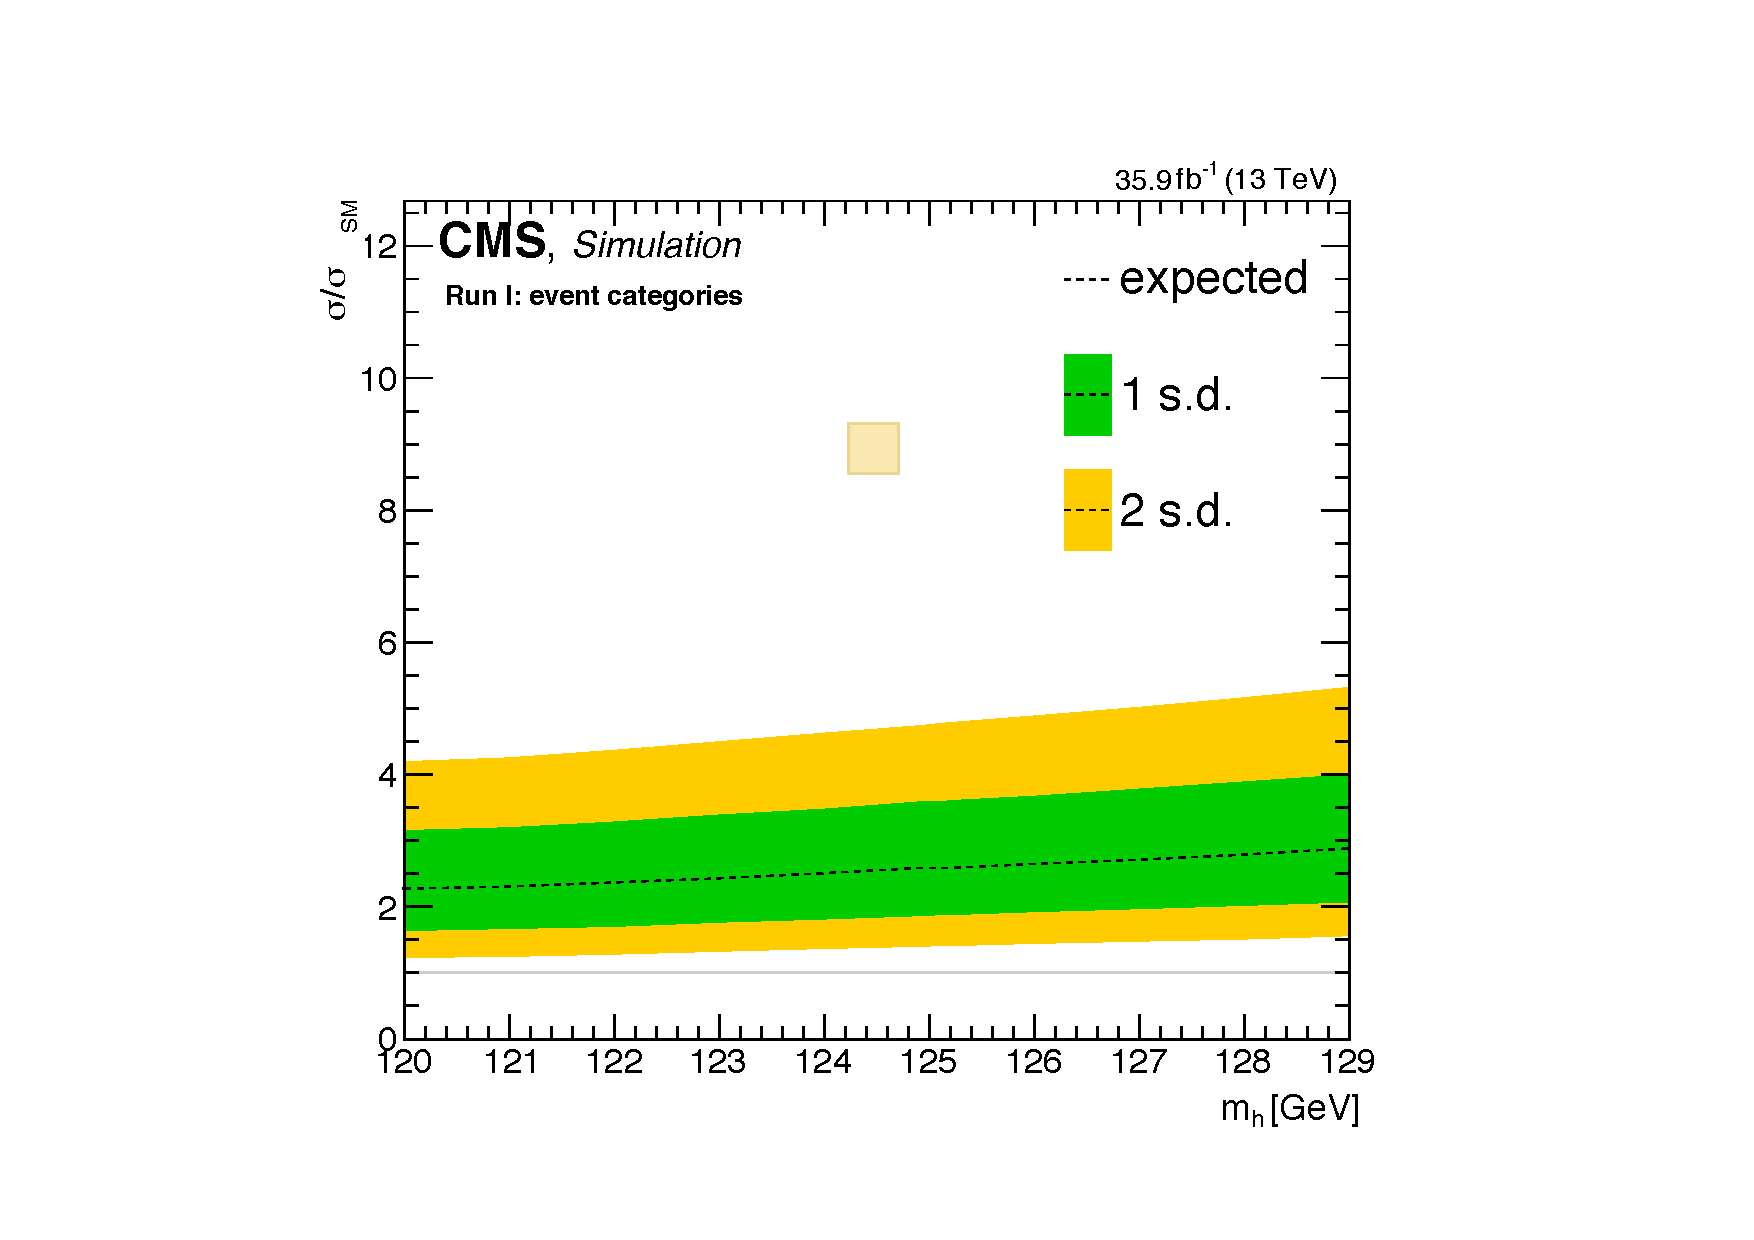
\includegraphics[width=0.8\textwidth]{figures/combine/limitsAsymptotic/baseline_110to160_p25GeV_NoNuis_Viktor/runIcat_b.pdf}
%      \caption{The combined 95\% CL expected exclusion limit computed using asymptotic approximation as a function of the probed Higgs boson mass for event categories as defined in Run~I analysis. Only statistical uncertainties are considered.}
%      \label{combine:LimitsAsymptotic}
%  \end{figure}
